\documentclass[a4paper]{article}
\usepackage[utf8]{inputenc}
\usepackage[russian,english]{babel}
\usepackage[T2A]{fontenc}
\usepackage[left=10mm, top=20mm, right=18mm, bottom=15mm, footskip=10mm]{geometry}
\usepackage{indentfirst}
\usepackage{amsmath,amssymb}
\usepackage[italicdiff]{physics}
\usepackage{graphicx}
\graphicspath{{images/}}
\DeclareGraphicsExtensions{.pdf,.png,.jpg}
\usepackage{wrapfig}
\usepackage{float}
\usepackage{subcaption}
\usepackage{enumitem}
\usepackage{caption}
\usepackage{array}
\captionsetup[figure]{name=Рисунок}
\captionsetup[table]{name=Таблица}

\title{\underline{Отчет о выполненой лабораторной работе 4.4.1}}
\author{Воронин Денис, Б04-407}

\begin{document}

\maketitle

\begin{center}
\textbf{\Large Изучение дифракционной решетки с помощью гониометра}
\end{center}

\textbf{Цель работы:}  Знакомство с работой и настройкой гониометра Г5,
определение спектральных характеристик амплитудной решётки.\par

\textbf{Оборудование:} гониометр, дифракционная решётка,
ртутная лампа.

\textbf{Аннотация:} отъюстрируем гониометр, исследуем спектр ртутной лампы, и дисперсию решетки в разных порядках, 
определим период и спектральные характеристи решеткиЮ оценис влияние ширины пучка на разрешающую способность.

\section{Теоретические сведения}

Основное соотношение приближенной теории дифракционной решётки:

	\begin{equation}
	d\sin \varphi_m = m\lambda.
 \label{main}
	\end{equation}
 
Угловая дисперсия $D$ характеризует угловое расстояние между близкими спектральными линиями:
	\begin{equation}
	D = \frac{d\varphi}{d\lambda} = \frac{m}{d \cos \varphi}=\frac{m}{\sqrt{d^{2}-m^{2} \lambda^{2}}}.
	\label{Dispersion}
	\end{equation}

Рассмотрим изображения спектра для двух узких спектральных линий с длинами волн $\lambda$ и $\lambda+\delta\lambda$. Для минимального значения $\lambda+\delta\lambda$, которое может быть определено по результатам измерений, вводят важнейшую характеристику спектрального прибора — разрешающую способность:

\begin{equation}
    R=\frac{\lambda}{\delta\lambda} = \frac{\varphi}{\delta \varphi}.
\end{equation}

\section{Экспериментальная установка}

\begin{figure}[H]
	\center{
\includegraphics[scale=0.1]{p1.png}}
  \caption{Экспериментальная установка}
	\label{fig:image1}
\end{figure}

Гониометр служит для точного измерения углов и находит широкое применение в оптических лабораториях. С помощью гониометра можно определять показатели преломления и преломляющие углы призм и кристаллов, исследовать параметры дифракционных решеток, измерять длины волн спектральных линии и т. д. В настоящей работе этот прибор применяется для исследования дисперсии стеклянных призм.

Гониометр Г5 состоит из следующих основных частей (рис. 4): коллиматора 3, столика 7, алидады 17 со зрительной трубой 12, которые крепятся на массивном основании 23. На столике 7 размещается исследуемый предмет (призма). Наклон столика относительно вертикальной оси регулируется винтами 8.

Коллиматор служит для получения параллельного пучка лучей. Он состоит из объектива 5 и щели 1, ширина которой (от 0 до 2 мм) регулируется микрометрическим винтом 2. Коллиматор крепится неподвижно на основании гониометра. Настройка коллиматора на параллельность пучка производится винтом 4.

Зрительная труба состоит из объектива 9 и окуляра 13. Объективы коллиматора и зрительной трубы одинаковы. Фокусировка трубы производится винтом 11. Наклон коллиматора и зрительной трубы к горизонтальной оси изменяется винтами 6 и 10 соответственно. В состав гониометра входит несколько окуляров, среди них окуляр-куб и окуляр Монченко.

Схема окуляра-куба зрительной трубы приведена на рис. 5, а. Свет от лампы Л проходит защитную стеклянную пластинку П и попадает на автоколлимационную сетку А, содержащую две взаимно перпендикулярные щели (рис. 5, б). Свет, прошедший через сетку, попадает на две прямоугольные призмы Р, на гипотенузные грани которых нанесен полупрозрачный слой с коэффициентом отражения 50 \%.

\begin{figure}[H]
	\center{
\includegraphics[scale=0.8]{p2.png}}
  \caption{Экспериментальная установка}
	\label{fig:image1}
\end{figure}

\section{Ход работы}

\subsection{Настройка гониометра}

Согласно техническому описанию выполнили юстрировку гониометра и установили начало отсчета.

\subsection{Установка решетки}

\begin{wrapfigure}{l}{0.4\textwidth}  % l = слева, ширина картинки 40% от ширины текста
    \centering
    
\includegraphics[scale = 0.03]{p5.jpg} % замените на ваше имя файла
    \caption{Щель}
    \label{fig:example}
\end{wrapfigure}

\textbf{1.} Настроили зрительную трубу на наблюдение входной щели коллиматора и настроили вертикальный размер изображения щели так, что она занимает не менее четверти поля зрения трубы.\par

Установили решетку так, стобы ее плоскость была параллельна одному из винтов 8 и перпендикулярна оси коллиматора.
Вращая верхнюю часть столика найдем ахроматическое ихображение щели коллиматора - спектр нулевого порядка.
\par

\textbf{2.} Отводя алидаду в сторону от коллиматора, найдем в трубе спектр самого дальнего порядка и винтом снова приведем изображение щели к центру.\par

Повторяя процедуру, методом последовательных приближений добъемся того, чтобы при повороте трубы изображение щели и спектр уходили не больше, чем на треть радиуса поля зрения.

\subsection{Исследование спектра ртутной лампы}

\begin{figure}[H]
	\center{
\includegraphics[scale=0.8]{p3.png}}
  \caption{Спектр ртутной лампы ДРШ}
	\label{fig:image1}
\end{figure}

\begin{figure}[H]
	\center{
\includegraphics[scale=0.8]{p4.png}}
  \caption{Характеристики спектра ртутной лампы ДРШ}
	\label{fig:image1}
\end{figure}

\textbf{3.} Подберем ширину входной щели так, стобв ширина желтой спектральной линии была чуть больше промежутка между линиями двойного штриха окуляра зрительной трубы.

\textbf{4.} Убедились, что для двух ярких линий спектра в одном порядке выполнено: $dsin\varphi_{m} \sim \lambda $.

\textbf{5.} Измерим угловые координаты спектральных линий ртути в $\pm 1$ порядках:

\par

Ноль: $180^{\circ}31'40''$

\begin{figure}[H]
	\center{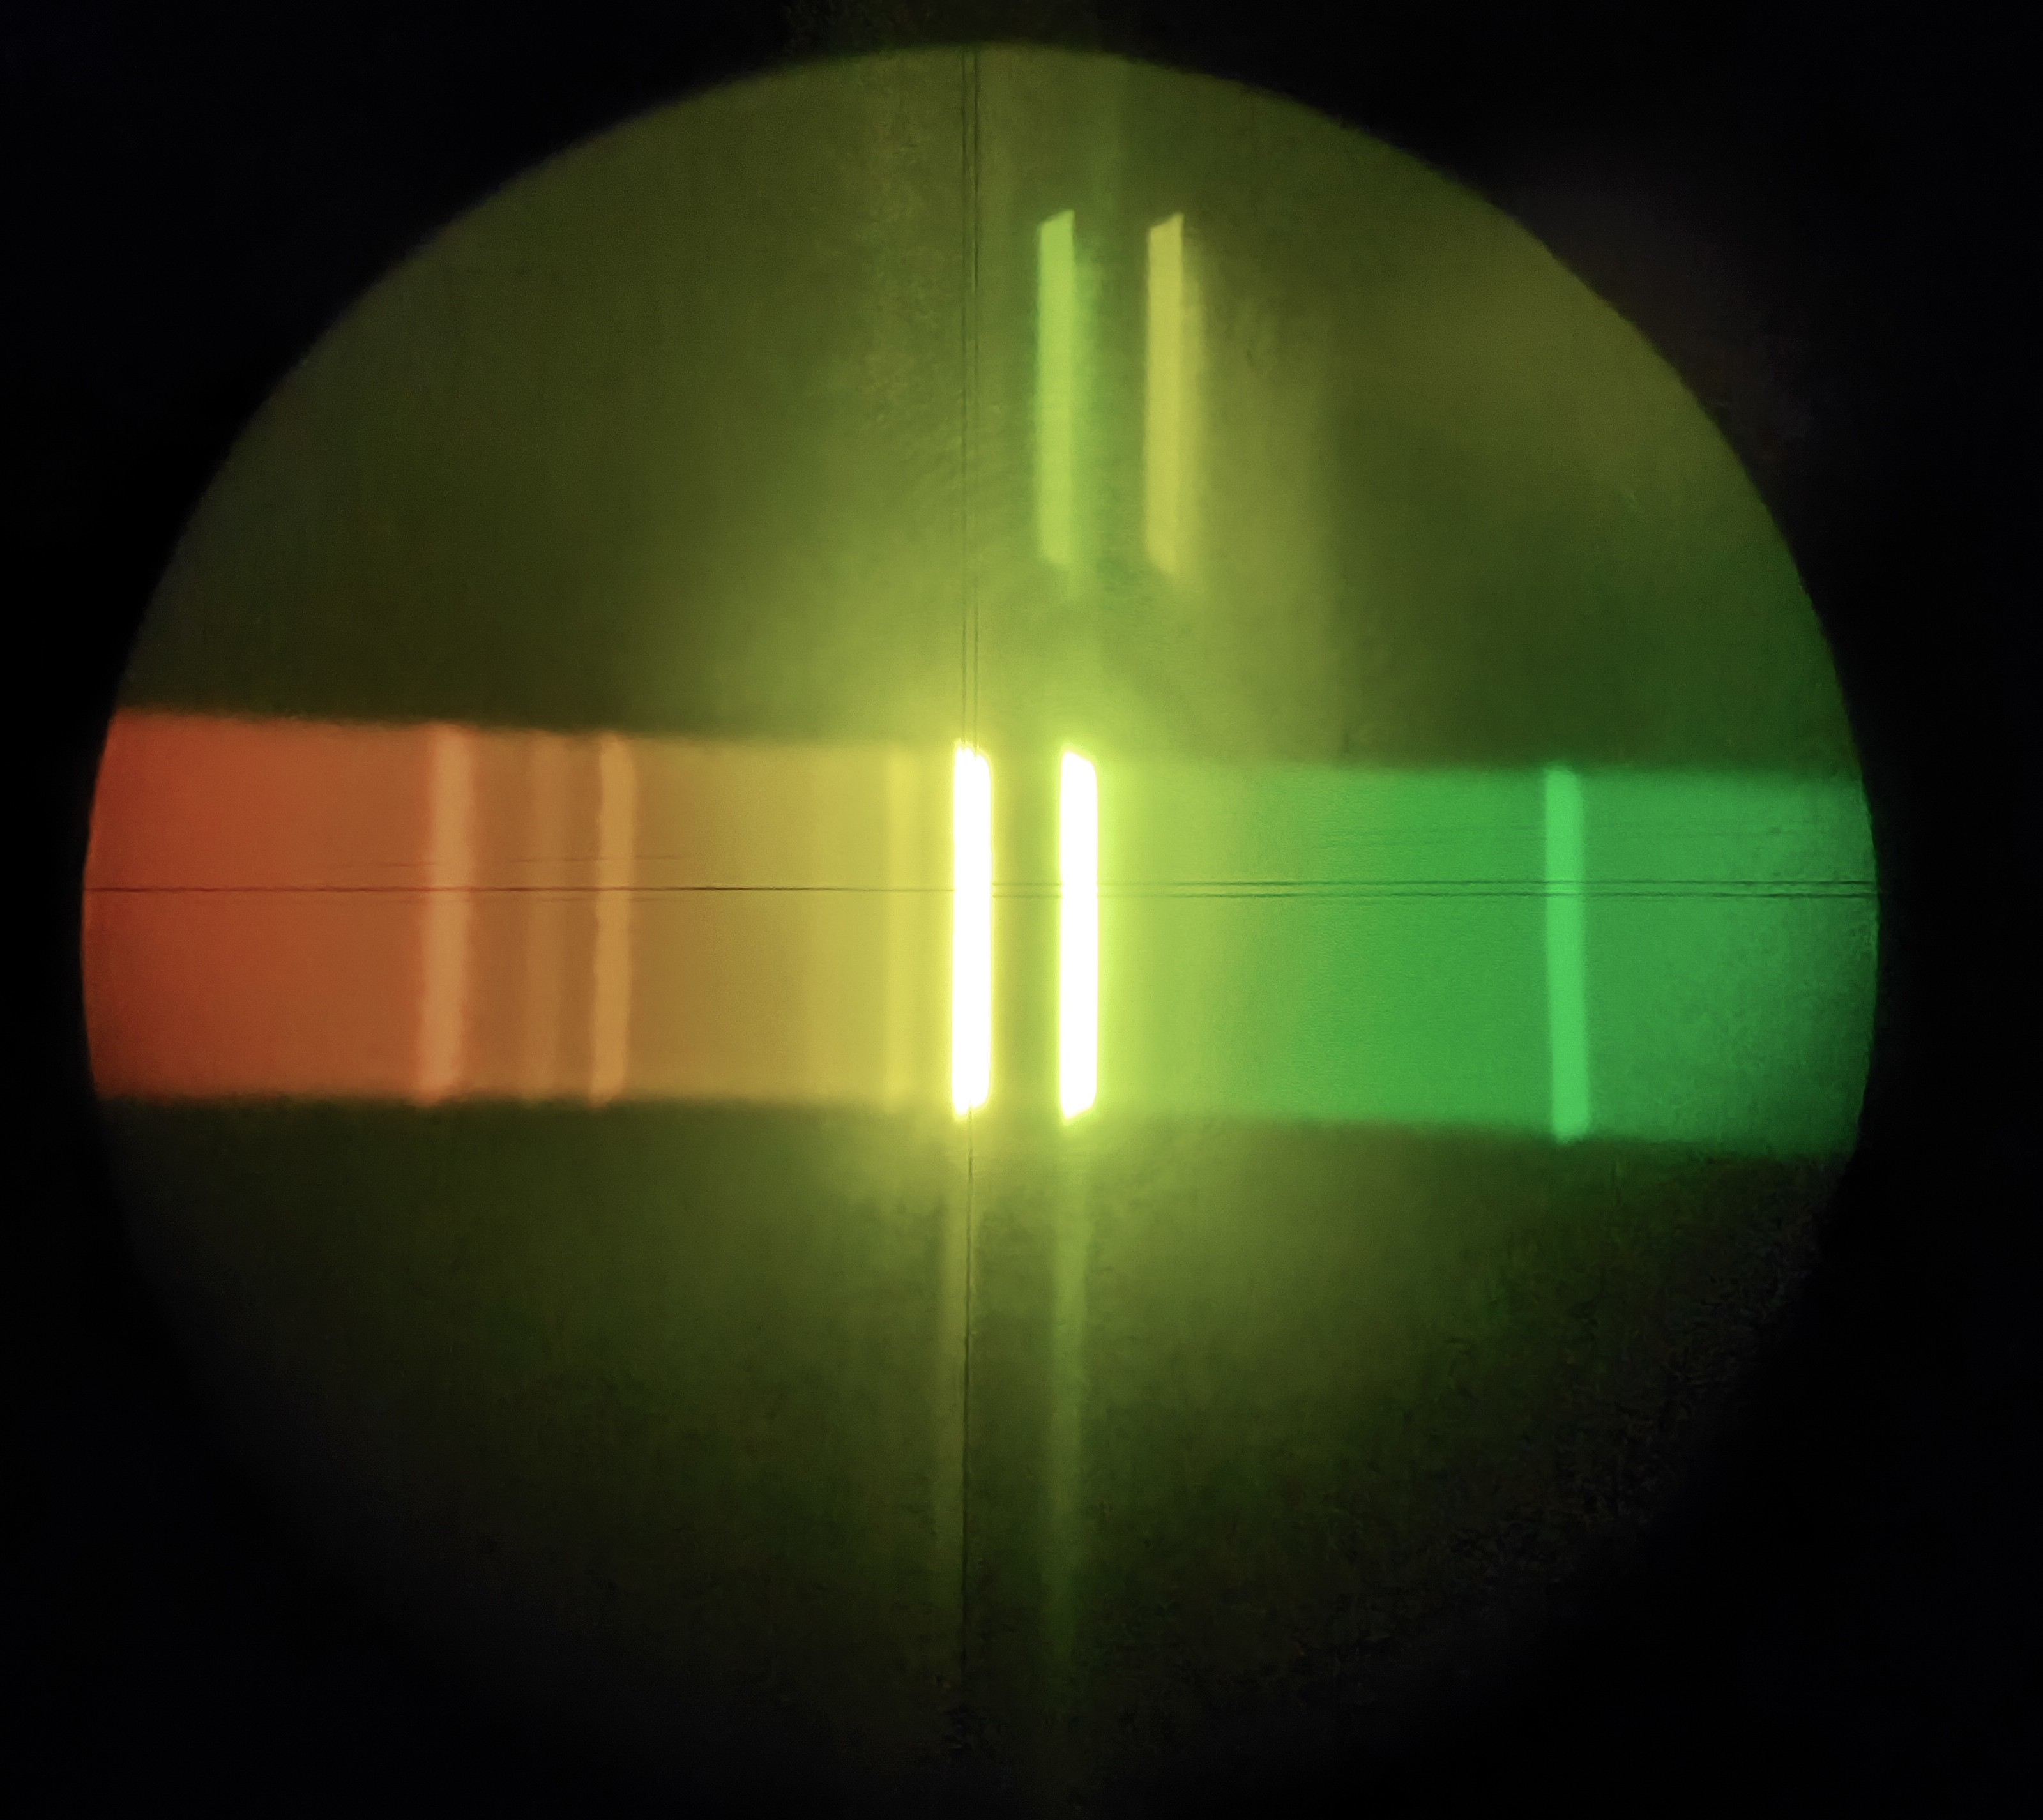
\includegraphics[scale=0.07]{p6.jpg}}
  \caption{Спектр}
	\label{fig:image1}
\end{figure}

Порядок m = 1:

\begin{tabular}{|c|c|c|c|c|c|c|c|c|}
\hline
Спектр  & K1 & K2 & 1 & 2 & 3 & 4 & 5 & 6 \\
\hline
Координата  & $162^{\circ}25'39''$ & $162^{\circ}34'49''$ & $163^{\circ}24'24''$ & $163^{\circ}28'26''$ & $164^{\circ}22'46''$ & $164^{\circ}59'46''$ & $167^{\circ}37'52''$ & $168^{\circ}31'40''$ \\
\hline
\end{tabular}

Порядок m = -1:

\begin{tabular}{|c|c|c|c|c|c|c|c|c|}
\hline
Спектр  & K1 & K2 & 1 & 2 & 3 & 4 & 5 & 6 \\
\hline
Координата  & $198^{\circ}52'39''$ & $197^{\circ}53'51''$ & $197^{\circ}5'40''$ & $197^{\circ}1'49''$ & $196^{\circ}6'5''$ & $194^{\circ}28'21''$ & $192^{\circ}45'51''$ & $191^{\circ}52'5''$ \\
\hline
\end{tabular}

\textbf{6.} Оценим угловую дисперсию решетки с помощью координат линий желтой пары во всех видимых порядках спектра:

\begin{tabular}{|c|c|c|c|c|c|}
\hline
m & $\varphi_1$ & $\varphi_2$ & $\Delta\varphi$ & D, arcsec/\AA & $\sigma_D$ \\
\hline
1 & $163^\circ 24' 24''$ & $163^\circ 28' 26''$ & $244''$ & 11.62 & 0.3 \\
\hline
-1 & $197^\circ 5' 40''$ & $197^\circ 1' 40''$ & $240''$ & 11.43 & 0.3 \\
\hline
2 & $145^\circ 9' 39''$ & $145^\circ 0' 41''$ & $538''$ & 25.62 & 0.6 \\
\hline
-2 & $215^\circ 46' 39''$ & $215^\circ 38' 20''$ & $499''$ & 23.76 & 0.8 \\
\hline
3 & $121^\circ 4' 59''$ & $120^\circ 44' 9''$ & $1250''$ & 59.52 & 0.7 \\
\hline
-3 & $241^\circ 24' 20''$ & $241^\circ 0' 10''$ & $1450''$ & 69.05 & 0.7 \\
\hline
\end{tabular}


\textbf{7.} Определим аппаратную разрешающую способность примерно: $R = \frac{5000}{2} = 2500$

\section{Обработка результатов}

\textbf{1.} Построим график для зависимости $sin\phi_{m}$ от $\lambda$ определим по коэффициенту наклона шаг решетки d:

\begin{figure}[H]
	\center{
\includegraphics[scale=0.5]{F1.png}}
  \caption{$sin\phi_{m}$ от $\lambda$}
	\label{fig:image1}
\end{figure}

Тогда $d = \frac{1}{2.5496* 10^{-5}\text{нм}} = 1.96 \pm 0.17\text{мкм}$

\textbf{2.} Рассчитаем экспериментальную угловую дисперсию для желтой пары в спектрах разных порядках $D = \frac{\Delta \varphi }{\Delta \lambda }$ и построим график зависимости D = f(m).

\begin{figure}[H]
	\center{
\includegraphics[scale=0.5]{F2.png}}
  \caption{$sin\phi_{m}$ от $\lambda$}
	\label{fig:image1}
\end{figure}

\textbf{3.} Рассчитаем экспериментальную разрешающую способность и сравнив ее с теоретической оценим число эффективно работающих штрихов и размер освещенной чпсти решетки:

\par

Так, измеренная угловая ширина одной из жёлтых полос первого порядка($\varphi = 17^\circ 5' 10'')$ составила $\delta \varphi = 2' 5'' = 125''$. Тогда получается $R \simeq 490$, а количество рабочих штрихов $N = R\cdot m = 492$, размер освещённой части $l = N \cdot \simeq 984$ мкм.

\textbf{4.} Рассчитаем порядок спектра, при котором фиолетоваялиния наложится на желтую:

\par

$m_\text{ж} \lambda_\text{ж} = m_\text{ф} \lambda_\text{ф}$ при слиянии. Тогда получается $m_\text{ж} = 7, m_\text{ф} = 10$.

\section{Вывод}

В ходе работы был изучен способ работы и настройки гониометра. Также с его помощью была проверена справедливость формулы (1), затем было получено значение периода дифракционной решётки($d = 1,96 \pm 0,17$ мкм), которое находится достаточно близко к истинному значению($d = 2$ мкм). Помимо этого, была также получена зависимость угловой дисперсии от порядка дифракции, которая затем, при сравнении с теоретической зависимостью, в некоторых точках даже совпала с ней. В конце концов, было получено значение разрешающей способности и при помощи неё затем оценены количество рабочих штрихов(490) и размер освещённой части(984 мкм).

\end{document}